\documentclass{article} % For LaTeX2e
\usepackage{iclr2026_conference,times}

\input{math_commands.tex}

\usepackage{hyperref}
\usepackage{graphicx}
\usepackage{booktabs}
\usepackage{amsmath,amssymb}
\usepackage{microtype}
\usepackage{subcaption}
\usepackage{enumitem}
\usepackage{array}
\graphicspath{{figures/}}

\hypersetup{
  colorlinks=true,
  linkcolor=blue,
  citecolor=blue,
  urlcolor=blue
}

\iclrfinalcopy

\title{Staged Metric-Gated GRPO Fine-Tuning Pipeline for Visual Numeric Reasoning}

\author{Kunal Ghosh\\
Purdue University\\
West Lafayette, Indiana, USA\\
\texttt{ghosh178@purdue.edu}\\
\texttt{kg.aero@gmail.com}}

\newcommand{\mcell}[1]{\begin{tabular}[t]{@{}l@{}}#1\end{tabular}}

\begin{document}

\maketitle
\fancyhead{}
\lhead{}
\chead{}
\rhead{}

\begin{abstract}
We study a staged metric-gated GRPO fine-tuning pipeline for visual numeric reasoning. The method combines a phase-wise curriculum over filtered MathVista subsets, a strict \texttt{<REASONING>} / \texttt{<SOLUTION>} response contract, metric-gated reward adaptation based on checkpoint evaluation, and alias-based checkpoint selection for non-monotonic training trajectories. We evaluate a rank-8 LoRA adaptation of \texttt{Qwen2.5-VL-7B-Instruct} under a fixed memory-constrained runtime profile. On the full \texttt{eval\_overall\_numeric} subset of MathVista \texttt{testmini} ($456$ examples), the best Phase B checkpoint improves exact match from $17.98\%$ to $49.78\%$, tolerance accuracy from $18.20\%$ to $50.66\%$, parseability from $25.44\%$ to $97.81\%$, and composite score from $11.63\%$ to $59.46\%$ relative to the baseline adapter evaluated under the same decoding protocol. These results suggest that curriculum staging, metric-gated reward control, and checkpoint-aware continuation can substantially improve the stability of RL fine-tuning for multimodal numeric question answering.

\textbf{Code:} \url{https://github.com/kgaero/RL_GSPO_Qwen2.5_7B}
\end{abstract}

\section{Introduction}

Reinforcement-learning fine-tuning for language and vision-language models is often summarized as a direct mapping from reward design to improved accuracy. In multimodal settings, however, the optimization problem is more complex \citep{yuan2025vlcogito}. Before correctness reward becomes informative, the policy must already emit outputs that are parseable, non-truncated, and structurally compatible with the evaluator \citep{shen2025satori}. If those preconditions are unstable, RL updates can be difficult to interpret because an apparent correctness failure may in fact be a formatting or completion failure \citep{shen2025satori}.

This paper investigates a staged metric-gated GRPO fine-tuning pipeline for visual numeric reasoning using \texttt{Qwen2.5-VL-7B-Instruct} as the base VLM. The pipeline leaves the GRPO objective unchanged and augments fine-tuning with filtered curriculum stages, a strict response contract, rule-based reward adaptation keyed to checkpoint metrics, and checkpoint aliases that allow continuation from the best structural or composite checkpoint rather than always from the most recent one. We analyze how this fine-tuning pipeline produces a structure-first and correctness-later trajectory for multimodal numeric question answering.

The implementation is designed to be auditable: controller states are saved, checkpoint aliases are explicit, reward weights are persisted, and evaluation artifacts contain both aggregate and sample-level records. This instrumentation is valuable in constrained-compute RL settings, where structural failures dominate early training and continuation decisions materially affect outcomes.

Figure~\ref{fig:pipeline} summarizes the loop. A base VLM is prepared with LoRA adapters, fine-tuned on a stage-filtered phase mixture, evaluated checkpoint by checkpoint, and then fed back into a controller that updates reward weights after each checkpoint evaluation. Table~\ref{tab:stage-matrix} shows that the curriculum is implemented as overlapping filtered views over the same MathVista split rather than as disjoint datasets.

\paragraph{Contributions.}
\begin{enumerate}[leftmargin=1.2em]
\item We document a staged GRPO fine-tuning pipeline for visual numeric reasoning that explicitly prioritizes structure stabilization before the main correctness gains.
\item We formalize the metric-gated reward controller and checkpoint aliasing logic so they can be read as an auditable algorithm rather than as scattered implementation details.
\item We report a controlled full-evaluation comparison across Baseline, Phase A, Phase B, and Phase C checkpoints on the same numeric \texttt{testmini} evaluation subset, with the highest primary score obtained by Phase B.
\end{enumerate}

\begin{figure}[t]
\centering
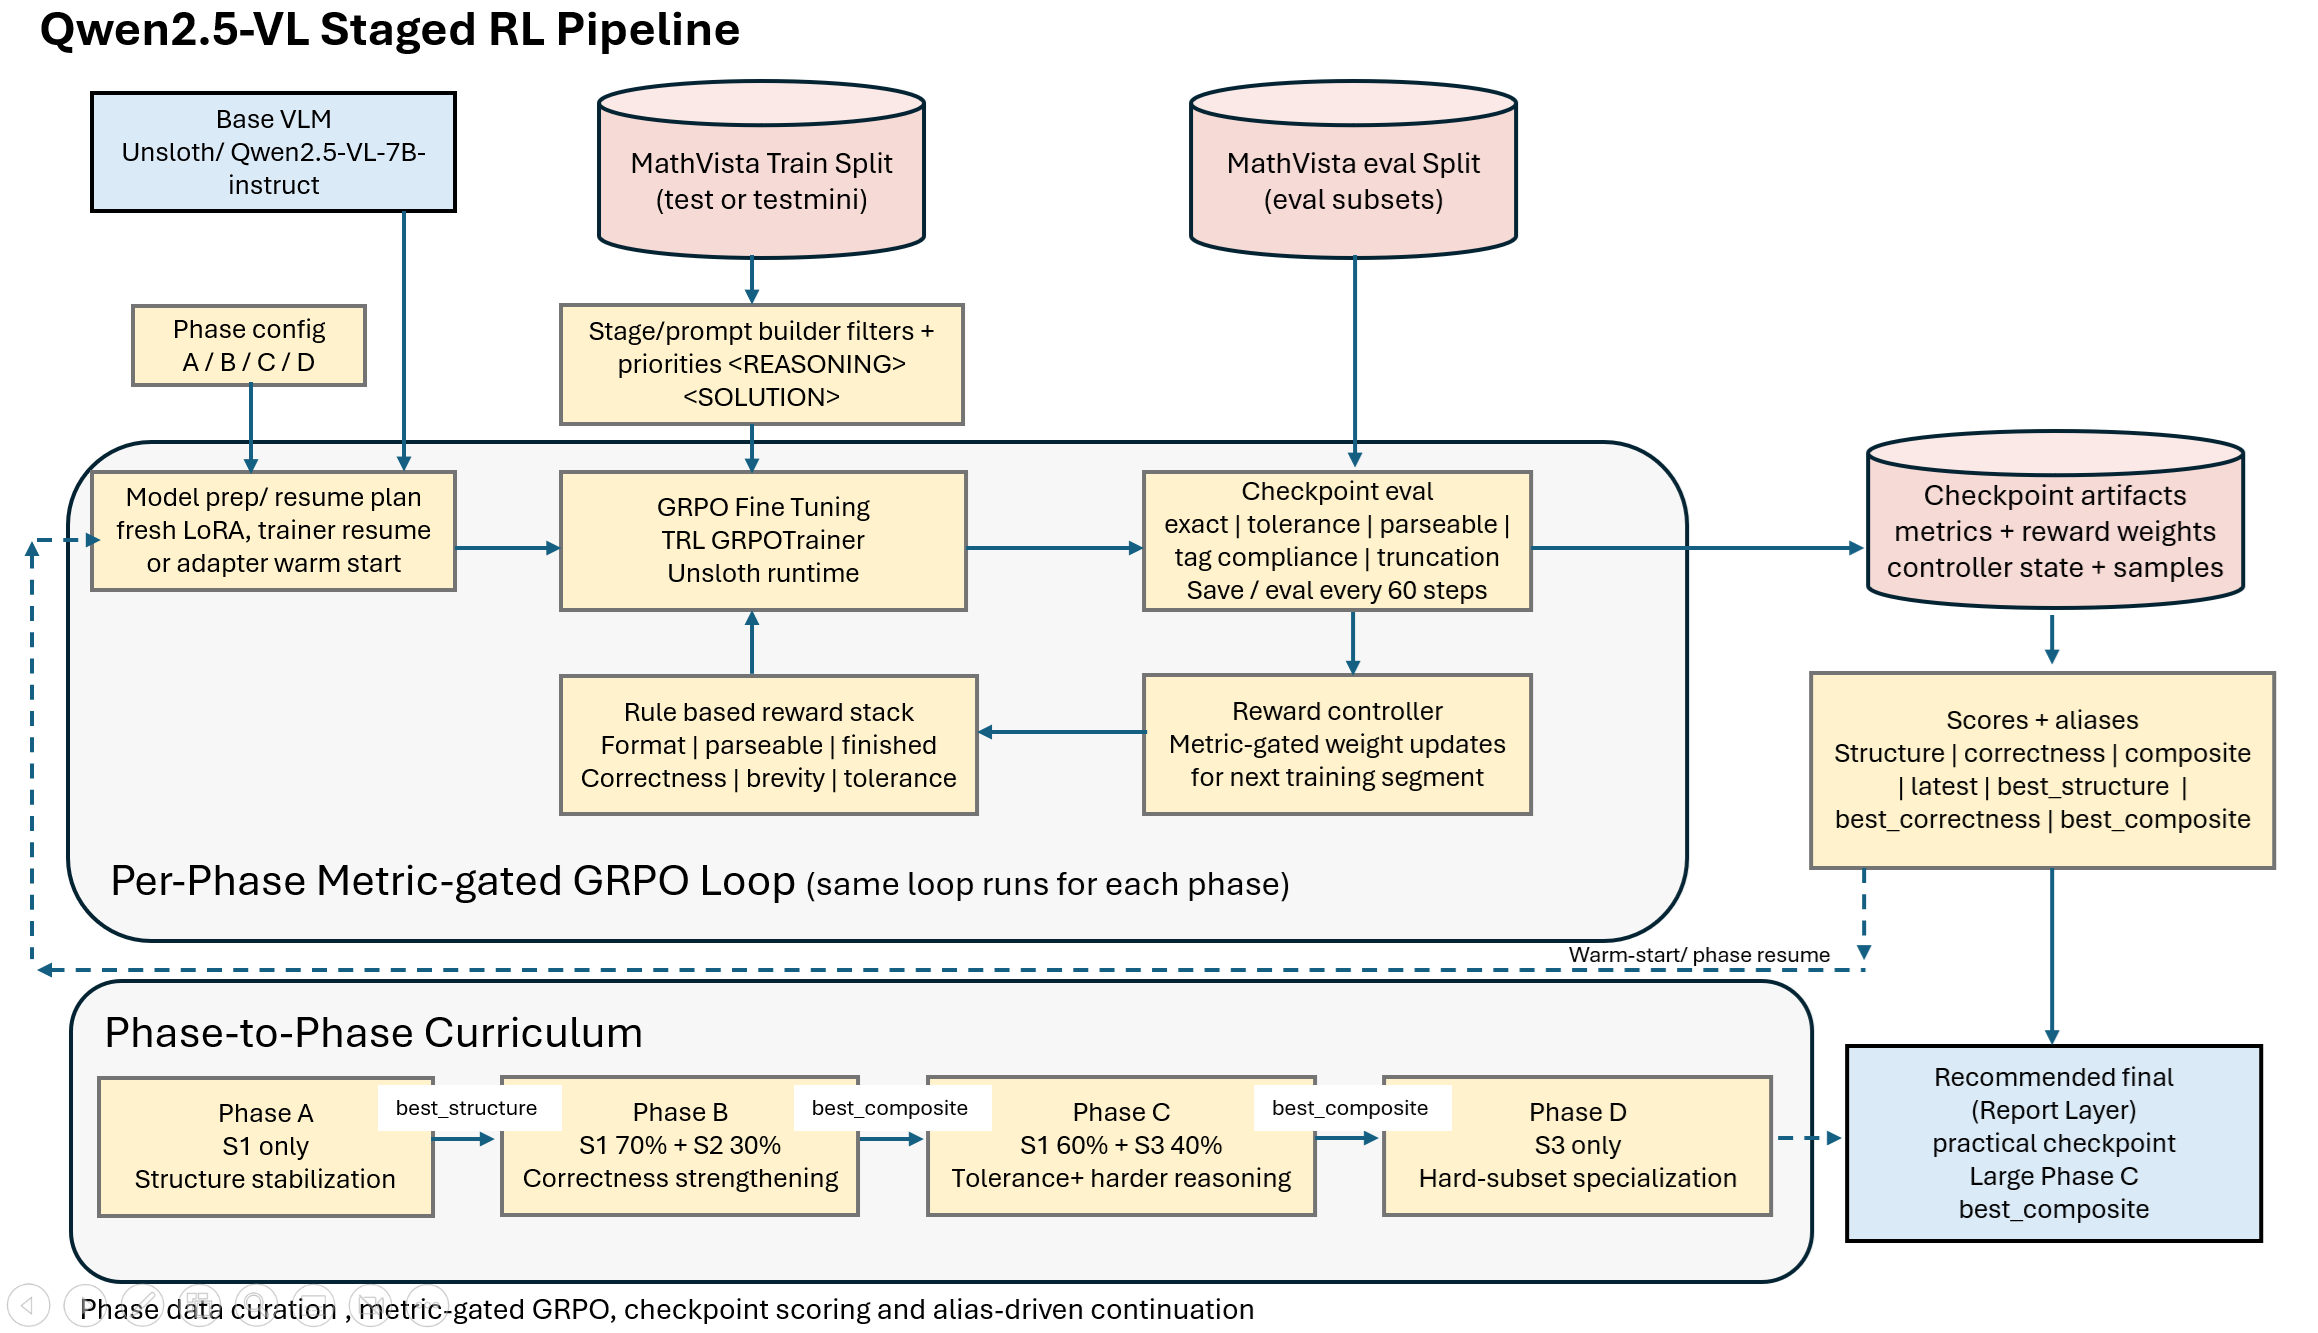
\includegraphics[width=\linewidth]{staged_training_pipeline_better.png}
\caption{Overview of the staged metric-gated GRPO loop. The pipeline couples phase-specific data curation, GRPO fine-tuning, checkpoint-side evaluation, reward-weight adaptation, and alias-based continuation. The method studied here is the fine-tuning pipeline around GRPO rather than a new GRPO loss.}
\label{fig:pipeline}
\end{figure}

\section{Related Work}

\paragraph{RL fine-tuning and preference optimization.}
Recent RLHF and preference-optimization work has primarily focused on new objectives or more efficient learning regimes. DeepSeekMath introduced GRPO as a group-relative alternative to PPO for mathematical reasoning \citep{deepseekmath2024}. SPPO and Asynchronous RLHF studied, respectively, self-play preference optimization and faster off-policy online RLHF \citep{wu2025sppo,noukhovitch2025async}. More recent multimodal post-training studies have adapted GRPO- or RL-style optimization to vision-language reasoning through cold-start supervision, staged reinforcement learning, and explicit reasoning incentives \citep{huang2025visionr1,wei2025coldstart,chen2025revisualr1}. Our contribution is complementary: we leave the underlying GRPO objective unchanged and study how a staged fine-tuning pipeline combines GRPO with curriculum scheduling, metric-gated reward adaptation, and checkpoint-selection logic in a failure-prone multimodal setting.

\paragraph{Multimodal mathematical reasoning.}
MathVista highlights the difficulty of mathematical reasoning in visual contexts and serves as a benchmark for diagram, chart, table, and numeric question answering behavior \citep{lu2024mathvista}. Recent work has addressed this problem with larger synthetic corpora, progressive curricula, staged reinforcement learning, or more explicit visual reasoning mechanisms \citep{zhang2025mavis,qi2025cogcom,liu2025infimmr,yuan2025vlcogito}. This paper focuses on the training-system side of the problem: a standard pretrained VLM paired with staged curricula, metric-gated reward control, and checkpoint-aware continuation that prioritize structural reliability before stronger correctness pressure.

\paragraph{Curriculum and adaptive reward control.}
Our approach is closest in spirit to curriculum and adaptive-control approaches that treat fine-tuning as a sequence of regimes rather than as one stationary objective. Recent multimodal reasoning work has explored phased reinforcement learning, progressive curriculum RL, and rubric-based curriculum design as mechanisms for stabilizing difficult reasoning behavior \citep{liu2025infimmr,yuan2025vlcogito,chen2026rucl}. The distinctive feature here is the granularity of adaptation: checkpoint metrics trigger reward changes directly within the fine-tuning pipeline.

\section{Problem Setup and Design Goals}

We study a policy $\pi_\theta(c \mid x)$ that maps a visual question-answering input $x$ to a completion $c$. Our method does not treat success as a single scalar notion of accuracy. Instead, it decomposes success into a sequence of preconditions:
\begin{enumerate}[leftmargin=1.2em]
\item the model must emit the required tagged structure,
\item the final answer must be parseable,
\item the answer must finish within the completion budget, and
\item the parsed answer must be correct under exact or tolerance-based matching.
\end{enumerate}
The central question is therefore not only how to optimize correctness, but also when correctness reward becomes informative enough to emphasize. If structure is unstable, correctness reward is sparse because malformed or truncated outputs never reach a meaningful matching stage.

The implementation makes three concrete design choices.
\begin{itemize}[leftmargin=1.2em]
\item \textbf{Increasing-difficulty data staging.} The policy first sees easier integer-valued numeric problems before harder float and geometry-heavy subsets are emphasized.
\item \textbf{Metric-gated rewards.} Reward weights change only after checkpoint evaluation, using measured failure modes rather than a fixed epoch schedule.
\item \textbf{Alias-based continuation.} Checkpoint continuation is based on structure, correctness, or composite aliases rather than assuming the latest checkpoint is best.
\end{itemize}
Taken together, these choices define the central design logic of the method.

\section{Method}

\subsection{Task, response contract, and phase structure}

The code targets MathVista-style visual question answering in which the answer is primarily numeric and free-form. Each prompt is wrapped with a strict output contract:
\begin{quote}
\small\ttfamily
<REASONING> ... </REASONING>\\
<SOLUTION> single numeric answer </SOLUTION>
\end{quote}
This contract is important because both the reward functions and the evaluator depend on extracting a unique solution string from the completion. The pipeline also contains a separate multi-choice scaffold, but that branch is disabled by default and is not part of the main evidence.

The curriculum is organized into stages and phases. Stages are filtered subsets over the same dataset. In the configuration used for the main training path:
\begin{itemize}[leftmargin=1.2em]
\item \textbf{Stage 1} restricts to easier English free-form integer questions on synthetic scenes, tables, and natural images.
\item \textbf{Stage 2} broadens to integer and float answers, adding tables, charts, plots, scientific figures, and natural images.
\item \textbf{Stage 3} emphasizes harder geometry, scientific-figure, plot, and abstract-scene problems.
\end{itemize}
Phases then mix these stages with different reward emphases:
\begin{itemize}[leftmargin=1.2em]
\item \textbf{Phase A}: Stage 1 only, structure stabilization.
\item \textbf{Phase B}: $0.7$ Stage 1 + $0.3$ Stage 2, early correctness strengthening.
\item \textbf{Phase C}: $0.6$ Stage 2 + $0.4$ Stage 3, harder reasoning and tolerance reward.
\end{itemize}

\begin{table}[t]
\centering
\setlength{\tabcolsep}{2pt}
\renewcommand{\arraystretch}{1.12}
\scriptsize
\begin{tabular}{>{\raggedright\arraybackslash}p{0.14\linewidth}>{\raggedright\arraybackslash}p{0.27\linewidth}>{\raggedright\arraybackslash}p{0.27\linewidth}>{\raggedright\arraybackslash}p{0.27\linewidth}}
\hline
\textbf{Filter} & \textbf{S1 Easy Numeric} & \textbf{S2 Medium / Float} & \textbf{S3 Hard Numeric} \\
\hline
Stage ID & \texttt{stage1\_easy\_numeric} & \texttt{stage2\_float\_numeric} & \texttt{stage3\_hard\_numeric} \\
\hline
Goal & easy numeric stabilization & moderate precision and broader numeric coverage & harder multistep numeric reasoning \\
\hline
Question type & \texttt{free\_form} & \texttt{free\_form} & \texttt{free\_form} \\
\hline
Answer type & \texttt{integer} & \texttt{integer}, \texttt{float} & \texttt{integer}, \texttt{float} \\
\hline
Language & \texttt{english} & \texttt{english} & \texttt{english} \\
\hline
Answer mode & \texttt{numeric\_free\_form} & \texttt{numeric\_free\_form} & \texttt{numeric\_free\_form} \\
\hline
Context families & \mcell{\texttt{synthetic scene}\\\texttt{table}\\\texttt{natural image}} & \mcell{\texttt{table}\\\texttt{chart}\\\texttt{plot}\\\texttt{scientific figure}\\\texttt{natural image}} & \mcell{\texttt{geometry diagram}\\\texttt{plot}\\\texttt{scientific figure}\\\texttt{abstract scene}} \\
\hline
Skills (any) & \mcell{\texttt{arithmetic reasoning}\\\texttt{statistical reasoning}\\\texttt{numeric commonsense}} & \mcell{\texttt{arithmetic reasoning}\\\texttt{statistical reasoning}\\\texttt{scientific reasoning}\\\texttt{numeric commonsense}} & \mcell{\texttt{geometry reasoning}\\\texttt{algebraic reasoning}\\\texttt{scientific reasoning}\\\texttt{arithmetic reasoning}\\\texttt{statistical reasoning}} \\
\hline
Hard only & False & False & True \\
\hline
\end{tabular}
\caption{Code-derived filter definitions for the three numeric curriculum stages used in the main training path. The stages overlap and are implemented as filtered views over the same MathVista split, not as fixed disjoint datasets.}
\label{tab:stage-matrix}
\end{table}

\subsection{Reward decomposition}

For a completion $c$, the method computes six per-sample reward components:
\begin{equation}
R(c)=\sum_{j=1}^{6} w_j r_j(c),
\end{equation}
where the components correspond to \texttt{format}, \texttt{parseable}, \texttt{finished}, \texttt{correctness}, \texttt{brevity}, and \texttt{tolerance}. The initial weights are phase-specific. Phase A places relatively high weight on structure and completion; Phase C raises correctness and activates tolerance reward.

The implementation never allows structure rewards to decay fully to zero. The guiding design principle is that, even when exact match becomes the main target, structural validity remains a necessary condition for receiving informative reward. The exact code-aligned reward definitions are reproduced in the supplement.

\subsection{Metric-gated reward control}

The reward controller updates weights after each checkpoint evaluation using explicit rules derived from observed metrics. Let $p$ denote parseable-answer rate, $s$ solution-tag compliance, $r$ reasoning-tag compliance, $m$ malformed rate, $t$ truncation rate, and $e$ exact match. The controller applies the following guards:
\begin{align}
p < 0.85 &\Rightarrow w_{\text{parseable}} \leftarrow \max(w_{\text{parseable}}, 0.75),\\
(s < 0.90)\ \vee\ (r < 0.88)\ \vee\ (m > 0.10) &\Rightarrow w_{\text{format}} \leftarrow \max(w_{\text{format}}, 0.75),\\
(t > 0.15)\ \vee\ (\bar{\ell} > 0.85L) &\Rightarrow w_{\text{finished}} \leftarrow w_{\text{finished}} + 0.25,
\end{align}
where $\bar{\ell}$ is average completion length and $L$ is the completion budget.

Correctness is escalated only when structure is already stable. Stability requires
\begin{equation}
p \ge 0.92,\quad s \ge 0.95,\quad r \ge 0.93,\quad m \le 0.05,\quad t \le 0.08,
\end{equation}
for a two-checkpoint window. If that condition holds and exact-match improvement over the window is below $0.02$, the controller increases correctness weight by $0.50$. All weights are then clamped to configured bounds. The rule set is intentionally simple enough to audit directly in saved checkpoint artifacts.

\subsection{Checkpoint-side evaluation and alias-based selection}

Instead of treating the most recent checkpoint as the default continuation point, the pipeline evaluates saved checkpoints and computes three aggregate scores:
\begin{align}
S_{\text{struct}} &= 0.35\,p + 0.20\,s + 0.20\,r - 0.15\,m - 0.10\,t, \\
S_{\text{corr}} &= 0.70\,e + 0.20\,a_{\text{tol}} + 0.10\,p, \\
S_{\text{comp}} &= 0.45\,e + 0.15\,a_{\text{tol}} + 0.15\,p + 0.10\,s + 0.05\,r - 0.05\,m - 0.05\,t,
\end{align}
where $a_{\text{tol}}$ is tolerance accuracy. These scores back four aliases: \texttt{latest}, \texttt{best\_structure}, \texttt{best\_correctness}, and \texttt{best\_composite}. Cross-phase continuation typically resumes from \texttt{best\_structure} or \texttt{best\_composite}, while same-phase restarts may use full trainer resume from \texttt{latest}. This distinction is important in the implementation because the code supports both full trainer-state restoration and LoRA-only warm start.

\section{Experimental Setting and Evaluation Protocol}

\paragraph{Dataset and model.} We use the Hugging Face release of MathVista, \texttt{AI4Math/MathVista} \citep{mathvista_hf,lu2024mathvista}, and load \texttt{unsloth/Qwen2.5-VL-7B-Instruct} as the base VLM \citep{unsloth_qwen25vl_hf,bai2025qwen25vl}.

\paragraph{Training protocol.}
The reported training trajectory uses the MathVista \texttt{test} split for Phase A--C fine-tuning. Phase A trains on Stage 1, Phase B trains on the configured Stage 1/2 mixture, and Phase C trains on the configured Stage 2/3 mixture. The selected checkpoints for final evaluation are \texttt{phase\_a/checkpoint-237}, \texttt{phase\_b/checkpoint-180}, and \texttt{phase\_c/checkpoint-240}.

\paragraph{Runtime profile.}
The main reported runs use the memory-constrained \texttt{kaggle\_t4} profile: 4-bit loading, LoRA rank $8$, max sequence length $1280$, image size $336$, gradient accumulation $4$, two sampled generations per prompt during RL fine-tuning, max prompt length $320$, and max completion length $64$. The trainer uses TRL's \texttt{GRPOTrainer} with sequence-level importance sampling and \texttt{dr\_grpo} loss.

\begin{table}[t]
\centering
\setlength{\tabcolsep}{3pt}
\renewcommand{\arraystretch}{1.15}
\scriptsize
\begin{tabular}{>{\raggedright\arraybackslash}p{0.34\linewidth}>{\raggedright\arraybackslash}p{0.20\linewidth}>{\raggedright\arraybackslash}p{0.34\linewidth}}
\hline
\textbf{Setting} & \textbf{Value} & \textbf{Used for} \\
\hline
LoRA rank / alpha / max rank & $8$ / $8$ / $8$ & all reported adapters and final evaluations \\
\hline
Model loading & 4-bit, max sequence length $1280$, image size $336$ & memory-constrained VLM loading \\
\hline
Training generation budget & max prompt length $320$, max completion length $64$ & Phase A--C GRPO fine-tuning \\
\hline
Training sampling & two generations per prompt & GRPO group-relative updates \\
\hline
Final evaluation sampling & one completion per prompt & primary comparison protocol except for generation sampling randomness \\
\hline
Final evaluation cap & no subset cap & full selected evaluation subsets \\
\hline
Primary subset & \texttt{eval\_overall\_numeric}, $456$ examples & main Baseline/A/B/C comparison \\
\hline
\end{tabular}
\caption{Runtime and evaluation settings used for the reported final comparison. The memory-constrained hardware profile contains a small evaluation cap by default, but the final evaluation explicitly clears that cap and evaluates the full selected subsets.}
\label{tab:t4-profile}
\end{table}

\paragraph{Final evaluation protocol.}
The primary comparison evaluates Baseline, Phase A, Phase B, and Phase C on the same MathVista \texttt{testmini} subset, \texttt{eval\_overall\_numeric}. The final evaluation uses one sampled completion per prompt, max completion length $64$, and no cap on the number of examples per subset. Stage-wise diagnostic evaluations are also computed on \texttt{stage1\_easy\_numeric}, \texttt{stage2\_float\_numeric}, and \texttt{stage3\_hard\_numeric}, but those diagnostics are not the primary metric.

\paragraph{Reproducibility.}
The implementation saves metrics, subset metrics, reward weights, controller state, controller decision logs, prompt-level records, and sample-level JSONL traces. The final evaluation artifacts include the primary-result CSV, stage-wise diagnostic CSV, subset-size JSON, and full JSON summary used to construct the tables below.

\section{Results}

\subsection{Full primary evaluation}

Table~\ref{tab:headline} reports the primary controlled comparison. The baseline adapter is evaluated with the same model runtime, LoRA shape, prompt contract, decoding budget, split, and evaluation subset as the trained adapters. Phase A produces the largest structural transition: parseability rises from $25.44\%$ to $98.90\%$ and composite score rises from $11.63\%$ to $58.59\%$. Phase B obtains the highest final exact match, tolerance accuracy, correctness score, and composite score. Phase C remains above baseline but does not improve over Phase B on the primary evaluation subset.

\begin{table}[t]
\centering
\small
\caption{Final full evaluation on \texttt{eval\_overall\_numeric} from MathVista \texttt{testmini} ($456$ examples).}
\label{tab:headline}
\begin{tabular}{llrrrrrrr}
\toprule
Phase & Checkpoint & Exact & Tol & Parse & AvgR & Struct & Corr & Comp \\
\midrule
Baseline & \texttt{baseline\_rank8} & 0.1798 & 0.1820 & 0.2544 & -0.0880 & 0.0285 & 0.1877 & 0.1163 \\
Phase A & \texttt{checkpoint-237} & 0.4803 & 0.4868 & \textbf{0.9890} & \textbf{6.3857} & 0.7421 & 0.5325 & 0.5859 \\
Phase B & \texttt{checkpoint-180} & \textbf{0.4978} & \textbf{0.5066} & 0.9781 & 5.8754 & 0.7371 & \textbf{0.5476} & \textbf{0.5946} \\
Phase C & \texttt{checkpoint-240} & 0.4737 & 0.4846 & \textbf{0.9890} & 6.0361 & \textbf{0.7436} & 0.5274 & 0.5833 \\
\bottomrule
\end{tabular}
\end{table}

\subsection{Improvement over baseline}

Table~\ref{tab:base-final} summarizes the highest-scoring primary checkpoint against the baseline. We report percentage-point gains rather than only relative gains because the baseline scores are low and relative changes can overstate the practical interpretation. The main result is a $31.80$ percentage-point exact-match gain and a $32.46$ percentage-point tolerance-accuracy gain at Phase B.

\begin{table}[t]
\centering
\small
\caption{Baseline versus the highest-scoring primary checkpoint, Phase B \texttt{checkpoint-180}.}
\label{tab:base-final}
\begin{tabular}{lrrr}
\toprule
Metric & Baseline & Phase B & Absolute Gain \\
\midrule
Exact match & 17.98\% & 49.78\% & +31.80 pp \\
Tolerance accuracy & 18.20\% & 50.66\% & +32.46 pp \\
Parseable rate & 25.44\% & 97.81\% & +72.37 pp \\
Average reward & -0.0880 & 5.8754 & +5.9634 \\
Structure score & 2.85\% & 73.71\% & +70.86 pp \\
Correctness score & 18.77\% & 54.76\% & +35.99 pp \\
Composite score & 11.63\% & 59.46\% & +47.83 pp \\
\bottomrule
\end{tabular}
\end{table}

\subsection{Reward trajectory during training}

Figure~\ref{fig:reward-vs-step} shows the mean training reward logged by the trainer across the selected Phase A, Phase B, and Phase C runs. The phase boundaries are aligned by cumulative training step. Because each phase uses different reward weights, the plot should be interpreted as a within-pipeline training diagnostic rather than as a direct evaluation metric. The main pattern is that Phase A rapidly reaches high structure-oriented reward, whereas Phases B and C operate under larger correctness pressure and therefore have lower absolute logged reward despite stronger downstream evaluation metrics.

\begin{figure}[t]
\centering
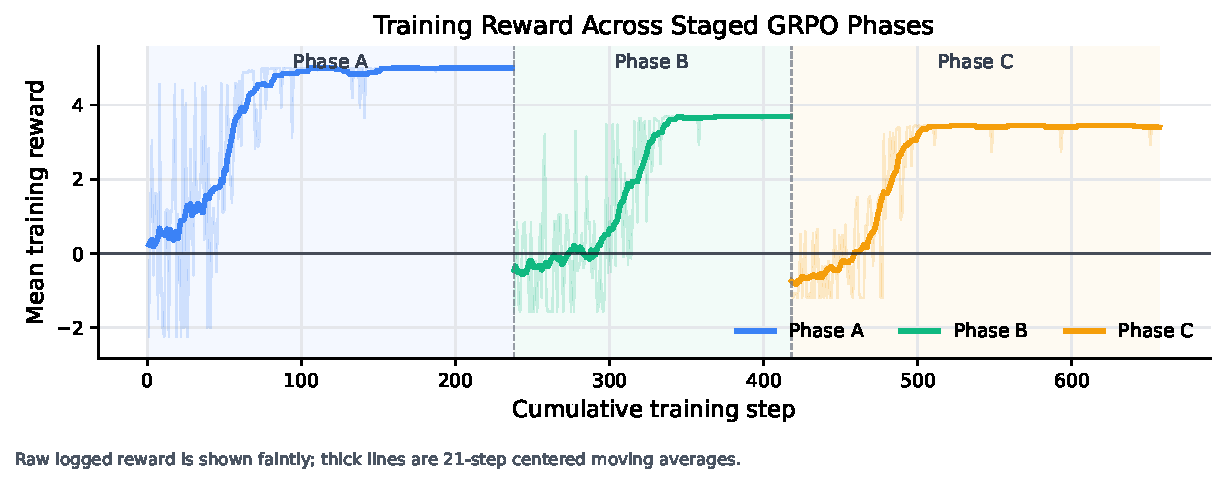
\includegraphics[width=0.95\linewidth]{reward_vs_step_phase_abc.pdf}
\caption{Training reward across the selected Phase A--C runs. Faint lines show raw per-step logged reward values from \texttt{trainer\_state.json}; thick lines show 21-step centered moving averages.}
\label{fig:reward-vs-step}
\end{figure}

\subsection{Stage-wise diagnostics}

The primary evaluation subset is identical for all four targets. Stage-wise subsets are used as diagnostics to understand where each checkpoint gains or loses behavior. Table~\ref{tab:stage-diagnostics} shows that all trained phases improve over baseline on every diagnostic subset. Phase B obtains the highest Stage 1 and Stage 2 exact match, while Phase C obtains the highest Stage 3 exact match. This pattern is consistent with the curriculum: Phase C emphasizes the Stage 2/3 mixture, but that specialization does not translate into the highest aggregate primary score.

\begin{table}[t]
\centering
\scriptsize
\caption{Stage-wise diagnostic evaluation on full \texttt{testmini} stage filters. These diagnostics are separate from the primary \texttt{eval\_overall\_numeric} comparison.}
\label{tab:stage-diagnostics}
\begin{tabular}{llrrrr}
\toprule
Phase & Eval subset & Exact & Tol & Parse & Trunc \\
\midrule
Baseline & Stage 1 & 0.1641 & 0.1641 & 0.2872 & 0.6923 \\
Baseline & Stage 2 & 0.1220 & 0.1220 & 0.1672 & 0.8293 \\
Baseline & Stage 3 & 0.0924 & 0.0924 & 0.1681 & 0.8151 \\
Phase A & Stage 1 & 0.4615 & 0.4615 & \textbf{0.9897} & 0.0051 \\
Phase A & Stage 2 & 0.4321 & 0.4460 & \textbf{0.9895} & 0.0000 \\
Phase A & Stage 3 & 0.3950 & 0.4034 & 0.9832 & 0.0084 \\
Phase B & Stage 1 & \textbf{0.4718} & \textbf{0.4718} & 0.9846 & 0.0000 \\
Phase B & Stage 2 & \textbf{0.4774} & \textbf{0.4983} & 0.9721 & 0.0035 \\
Phase B & Stage 3 & 0.3866 & 0.4118 & 0.9664 & 0.0000 \\
Phase C & Stage 1 & 0.4564 & 0.4564 & 0.9692 & 0.0000 \\
Phase C & Stage 2 & 0.4321 & 0.4530 & 0.9861 & 0.0000 \\
Phase C & Stage 3 & \textbf{0.4202} & \textbf{0.4286} & 0.9832 & 0.0000 \\
\bottomrule
\end{tabular}
\end{table}

\subsection{Structure improves before correctness}

The full evaluation supports the intended structure-first interpretation. The baseline produces many unparseable and truncated outputs, which makes correctness reward difficult to interpret. Phase A largely mitigates this failure mode: parseability becomes nearly saturated and average reward becomes strongly positive. Phase B then provides the highest correctness and composite scores. Phase C improves the hardest diagnostic subset but slightly reduces the aggregate primary metrics relative to Phase B.

This behavior is consistent with the controller design. Early reward pressure gives the model a stable response format and parseable final answer. Once that behavior is reliable, correctness and tolerance rewards become more informative. The non-monotonic Phase B to Phase C change also motivates alias-based checkpoint selection: later continuation is not guaranteed to dominate an earlier selected checkpoint on every evaluation view.

\begin{figure*}[p]
\centering
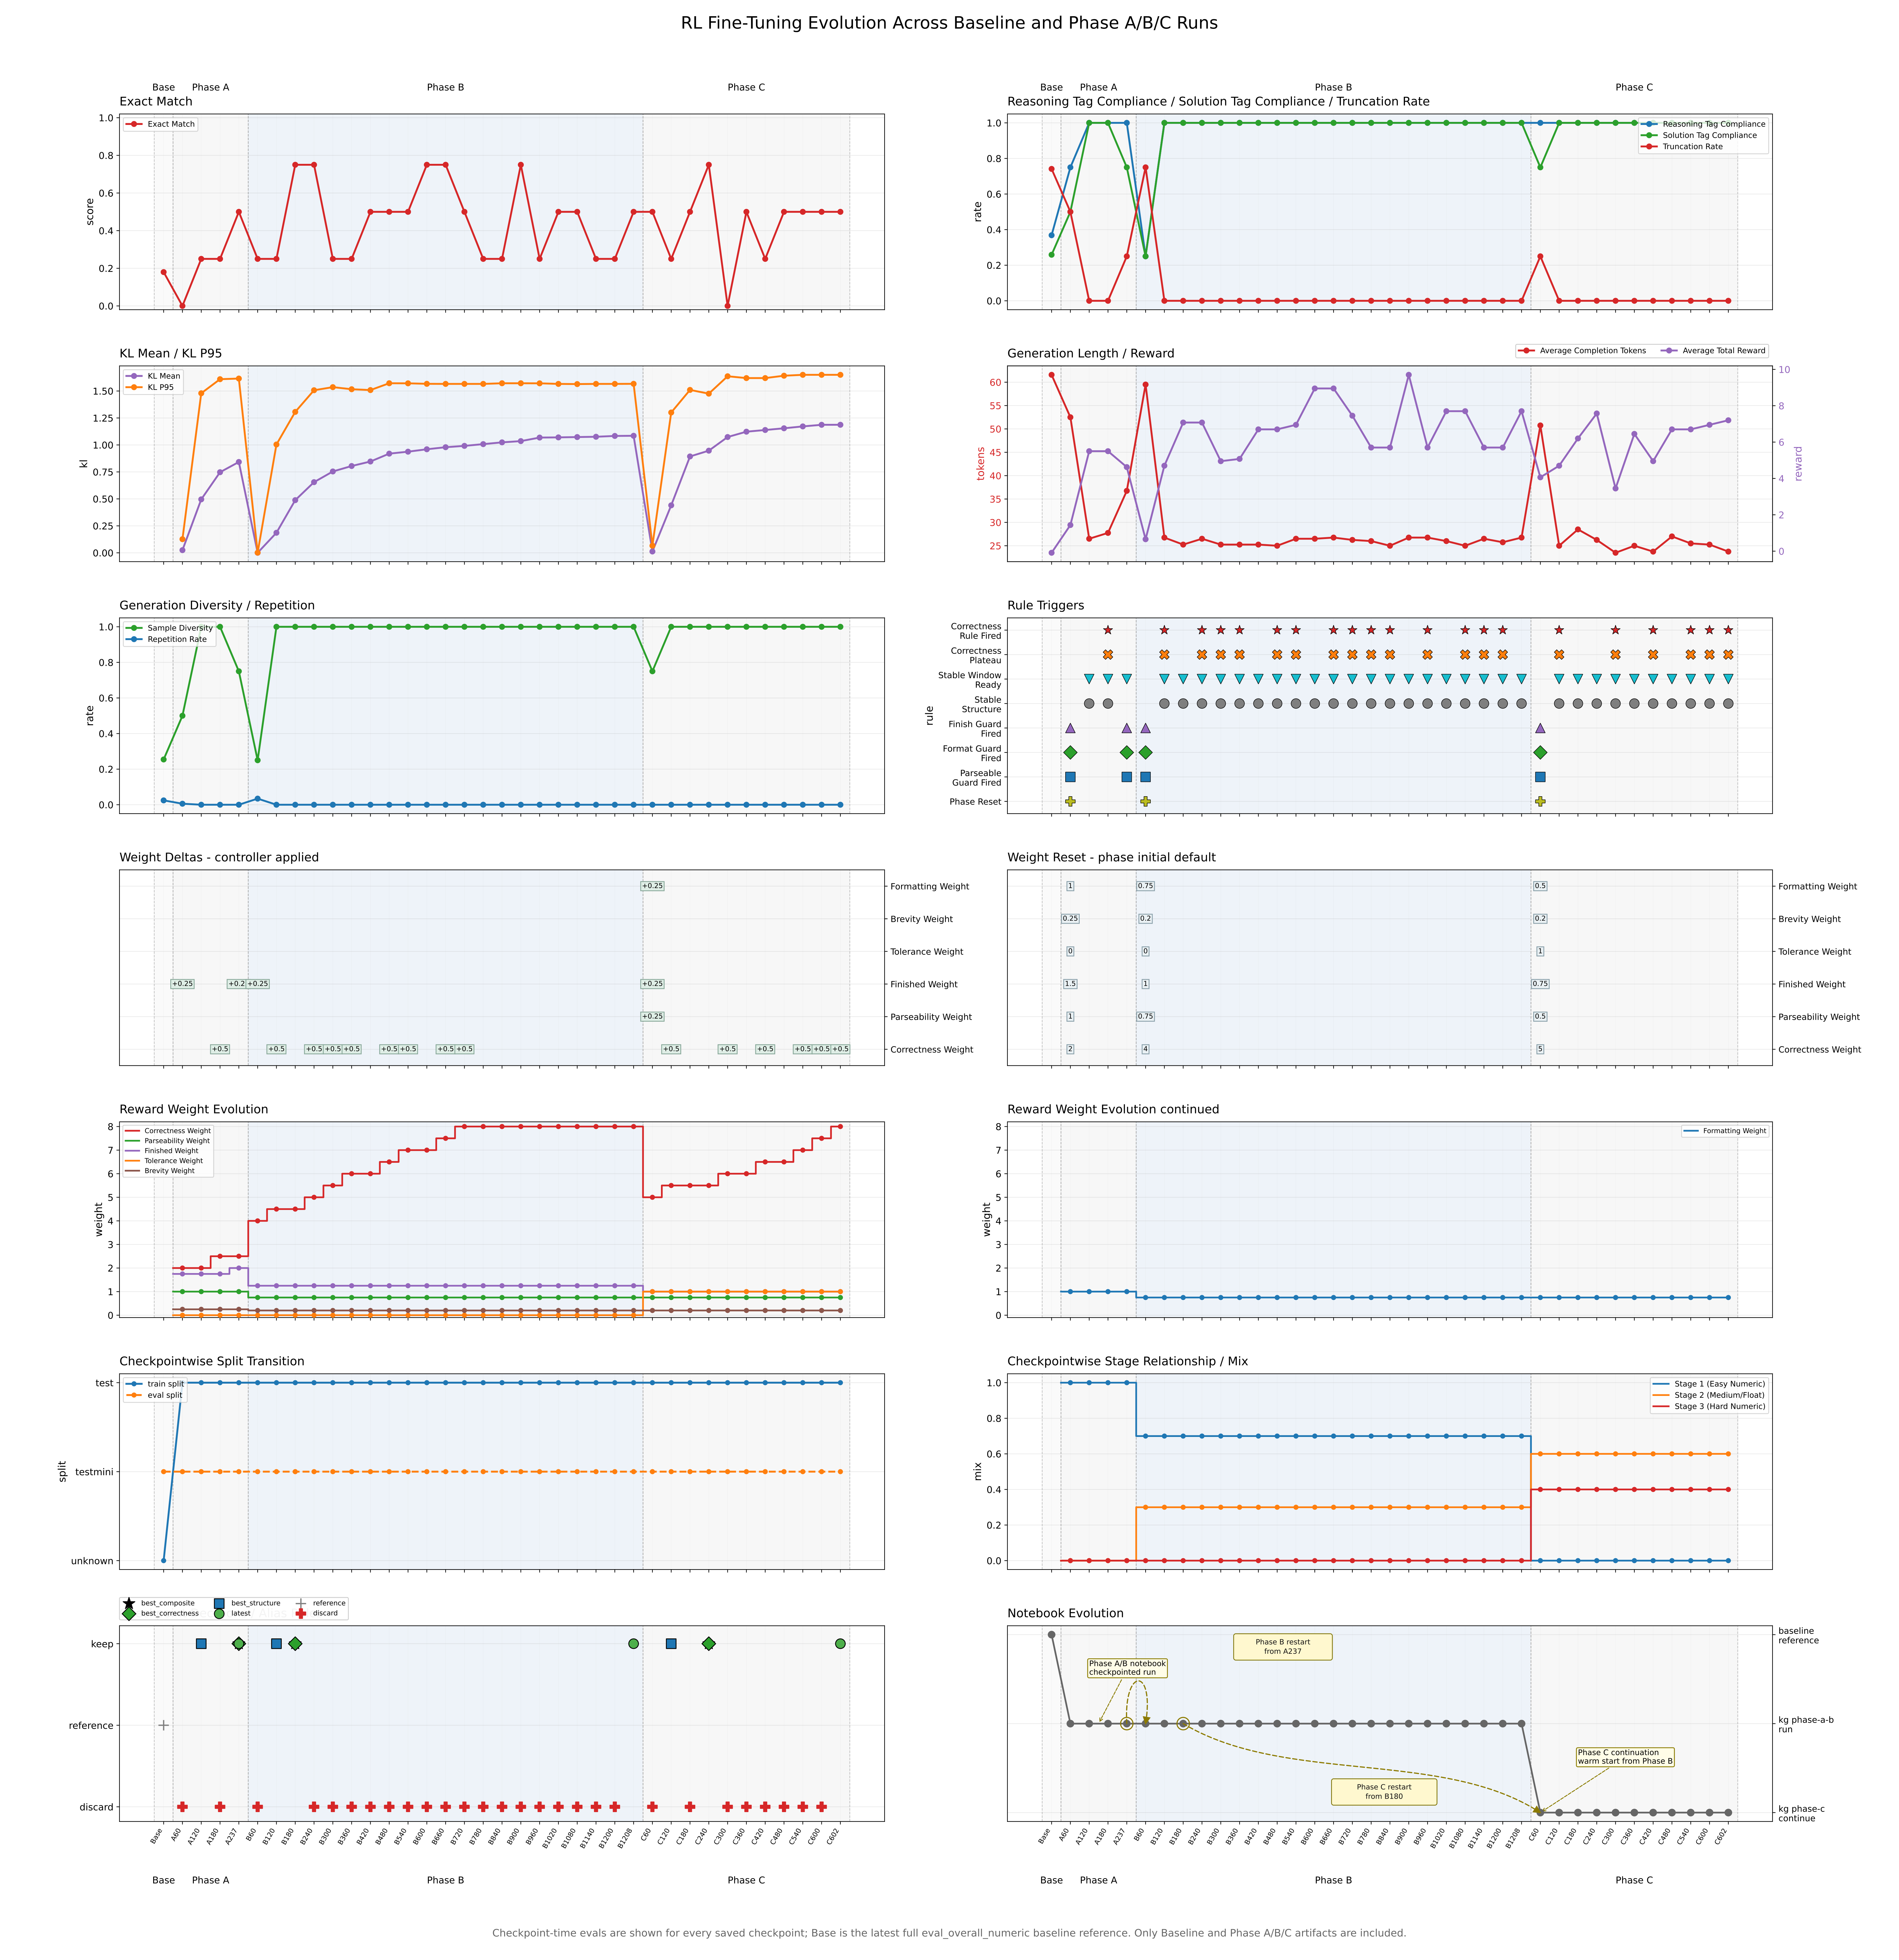
\includegraphics[width=\textwidth,height=0.9\textheight,keepaspectratio]{evolution_panels_notebook_paper.png}
\caption{Training evolution across checkpoint-side milestones. The reported primary result uses the full evaluation in Table~\ref{tab:headline}; this figure is retained as a qualitative view of the structure-first, correctness-later trajectory observed during training.}
\label{fig:evolution}
\end{figure*}

\section{Limitations and Reproducibility}

\begin{itemize}[leftmargin=1.2em]
\item The final primary evaluation uses the full numeric \texttt{testmini} subset, but it is still a single evaluation split with one sampled completion per prompt.
\item The reported runs use one base model family, one LoRA rank, one memory-constrained runtime profile, and no seed sweep.
\item Training uses the MathVista \texttt{test} split and evaluation uses \texttt{testmini}; broader held-out evaluation would be needed before making benchmark-level generalization claims.
\item Checkpoint selection is guided by checkpoint-side diagnostics, so future work should separate checkpoint selection and final reporting with an additional held-out validation split when compute permits.
\item The multi-choice branch and optional robustness stage have preliminary implementation support but are not part of the main evidence.
\end{itemize}

The study remains comparatively reproducible. It logs controller decisions at evaluated checkpoints, persists multiple checkpoint-selection aliases, saves sample-level traces, and includes unit tests for the most failure-prone logic. The supplement expands this record with explicit reward equations, evaluation formulas, controller thresholds, runtime settings, and transfer semantics.

\section{Conclusion}

We presented a staged metric-gated GRPO fine-tuning pipeline for visual numeric reasoning in a resource-constrained setting. The final full evaluation shows a substantial improvement over the baseline adapter: Phase B raises exact match from $17.98\%$ to $49.78\%$, tolerance accuracy from $18.20\%$ to $50.66\%$, parseability from $25.44\%$ to $97.81\%$, and composite score from $11.63\%$ to $59.46\%$ on the same $456$-example numeric \texttt{testmini} subset. The trajectory is structure-first and correctness-later: Phase A stabilizes output validity, Phase B gives the highest primary correctness, and Phase C improves the hardest diagnostic subset without improving the aggregate primary score. These findings support staged curriculum-based RL fine-tuning pipelines as a practical direction for multimodal numeric reasoning under constrained compute.

\bibliographystyle{iclr2026_conference}
\bibliography{references}

\end{document}
